% XXX Jedes Jahr Professoren-Texte aktualisieren!
\section[Eure Profs stellen sich vor]{Eure Professoren stellen sich vor}
\textbf{Auf den folgenden zwei Seiten stellen sich die Professoren vor, die Euch im integrierten Kurs Physik 1-3 betreuen werden. 
Die Theoretische Physik wird in diesem Kurs von Prof.\ Dr.\ Michael Klasen, die Experimentelle Physik von Prof.\ Dr.\ Martin Salinga vertreten. 
Die zugehörigen Übungen und Tutorien sowie das sehr nützliche Mathematik-Repetitorium werden von PD Dr.\ Karol Kovarik betreut. 
Prof.\ Dr.\ Lutz Hille wird in den ersten drei Semestern die Vorlesungen "Mathematik für Studierende der Physik" halten. Da Euch diese Professoren eine Zeit lang begleiten werden, ist es durchaus interessant zu wissen, was sie gemacht haben, bevor sie an die Universität Münster kamen, und womit sie sich in ihrer aktuellen Forschung beschäftigen.}

\begin{multicols}{2}
\begin{center} 
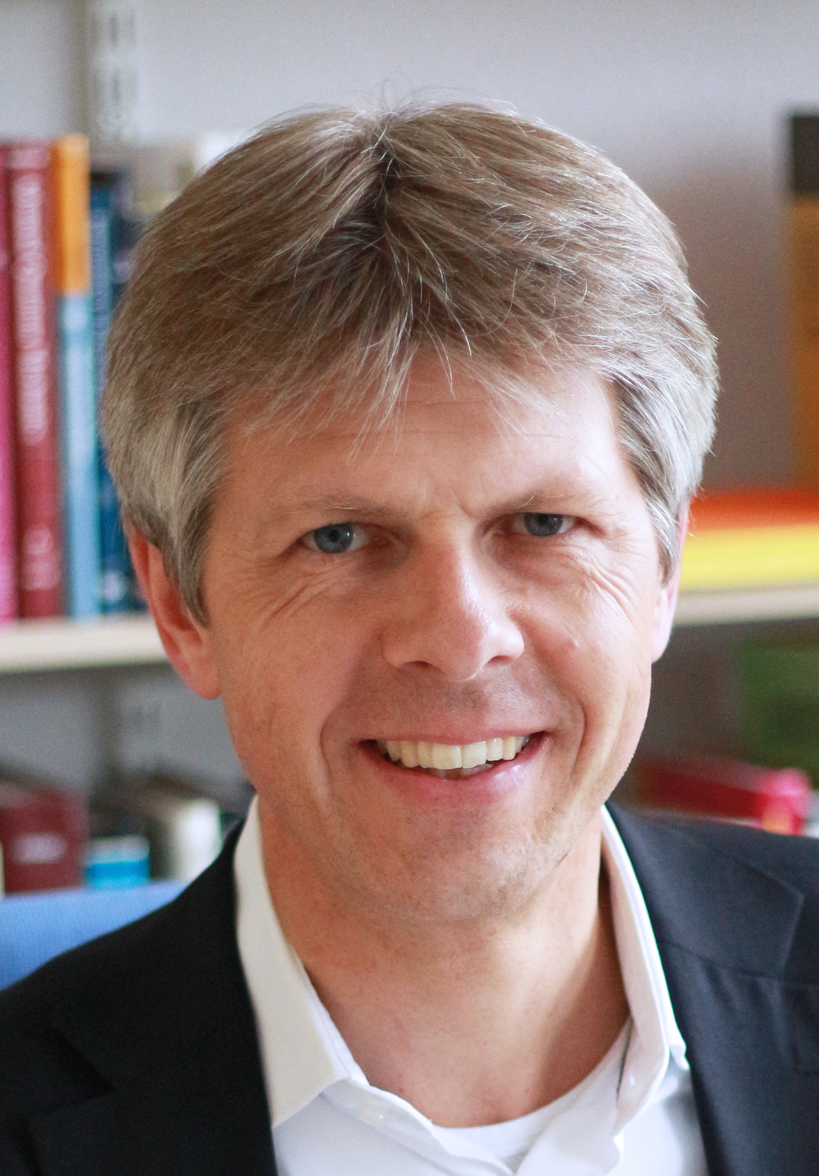
\includegraphics[width=0.8\columnwidth, height=0.25\textheight]{res/vorstellungsfotos/klasen_2016_5.jpg}
\smallskip
Prof.\ Dr.\ Michael Klasen\\ 
Institut für Theoretische Physik
\end{center} 

Herzlich willkommen an der Universität Münster, am Fachbereich Physik und in unserem integrierten Kurs Physik 1-3! Mein Kollege Martin Salinga und ich werden Ihnen gemeinsam die Grundlagen der Physik vermitteln und dabei das Zusammenwirken experimenteller Methoden und theoretischer Modellbildung herausstellen. Ein gutes Verständnis der Mathematik ist dabei besonders wichtig. 

Meine Alma Mater ist die Universität Würzburg, die - ähnlich wie wir jetzt - schon früh ein gut organisiertes Physikstudium, die Vermittlung von IT-Kompetenzen und zahlreiche Auslandskontakte, insbesondere in die USA, anbot. So verbrachte ich mein viertes Studienjahr an der Indiana University und konnte zum Bau eines kleinen Detektors für den dortigen Beschleuniger beitragen. Für Diplom- und Doktorarbeit wechselte ich 1992 in die Theoretische Physik und an die Universität Hamburg, wo ich Präzisionsrechnungen für den in diesem Jahr in Betrieb genommenen HERA-Kollider am Deutschen Elektronen-Synchrotron DESY durchführte. Nach der Promotion 1996 folgte ein Jahr am DESY, zwei Jahre am Argonne National Laboratory in Chicago, vier Jahre als Emmy-Noether-Gruppenleiter wieder in Hamburg und schließlich 2003 die Berufung auf eine Professur in Grenoble. In Münster bin ich seit 2011 und leite nun das Institut für Theoretische Physik. 

Die Physik fasziniert mich, weil sie als fundamentale Naturwissenschaft erklärt, was die Welt im Innersten zusammenhält. Teilchenphysik und Kosmologie führen uns an die Grenzen unseres Wissens und oft in die Nähe der Philosophie. Das spiegelt sich in der Forschung meiner Arbeitsgruppe, die vom Aufbau der Kernmaterie bis zur Rolle von Neutrinos und Dunkler Materie im frühen Universum reicht. Wichtig sind mir dabei immer die Genauigkeit der Rechnungen an der vordersten Front algebraischer und numerischer Methoden, meist auf Hochleistungsrechnern und unter zunehmendem Einsatz künstlicher Intelligenz, und die experimentelle Überprüfbarkeit der Ergebnisse. Die theoretischen Grundlagen bilden hierbei die relativistischen Quantenfeldtheorien der starken und elektroschwachen Wechselwirkung, das "Standardmodell der Teilchenphysik", aber auch hypothetische Modelle wie die Supersymmetrie und neue Theorien zur Erzeugung von Neutrinomassen und für die Erklärung Dunkler Materie. 

Relativitätstheorie und Quantenmechanik (die Physik des 20. Jahrhunderts) stehen auf den Schultern von Giganten, der klassischen Mechanik, Elektrodynamik und Thermodynamik. Diese Grundlagen werden wir uns in Physik 1-3 zunächst erarbeiten (müssen), um in Physik 4-6 die Quantenwelt und schließlich die Teilchenphysik und die Kosmologie zu verstehen. Von Beginn an werden wir aber die Konsequenzen der klassischen für die moderne Physik und die Bezüge zu aktuellen Fragen herausstellen. 

Ich wünsche Ihnen ganz herzlich einen guten Start für Ihr Studium, viele gute neue Freunde, tolle Erfahrungen und Eindrücke, viel Erfolg und ganz viel Spaß an der Physik!

\end{multicols}
%\begin{center}
%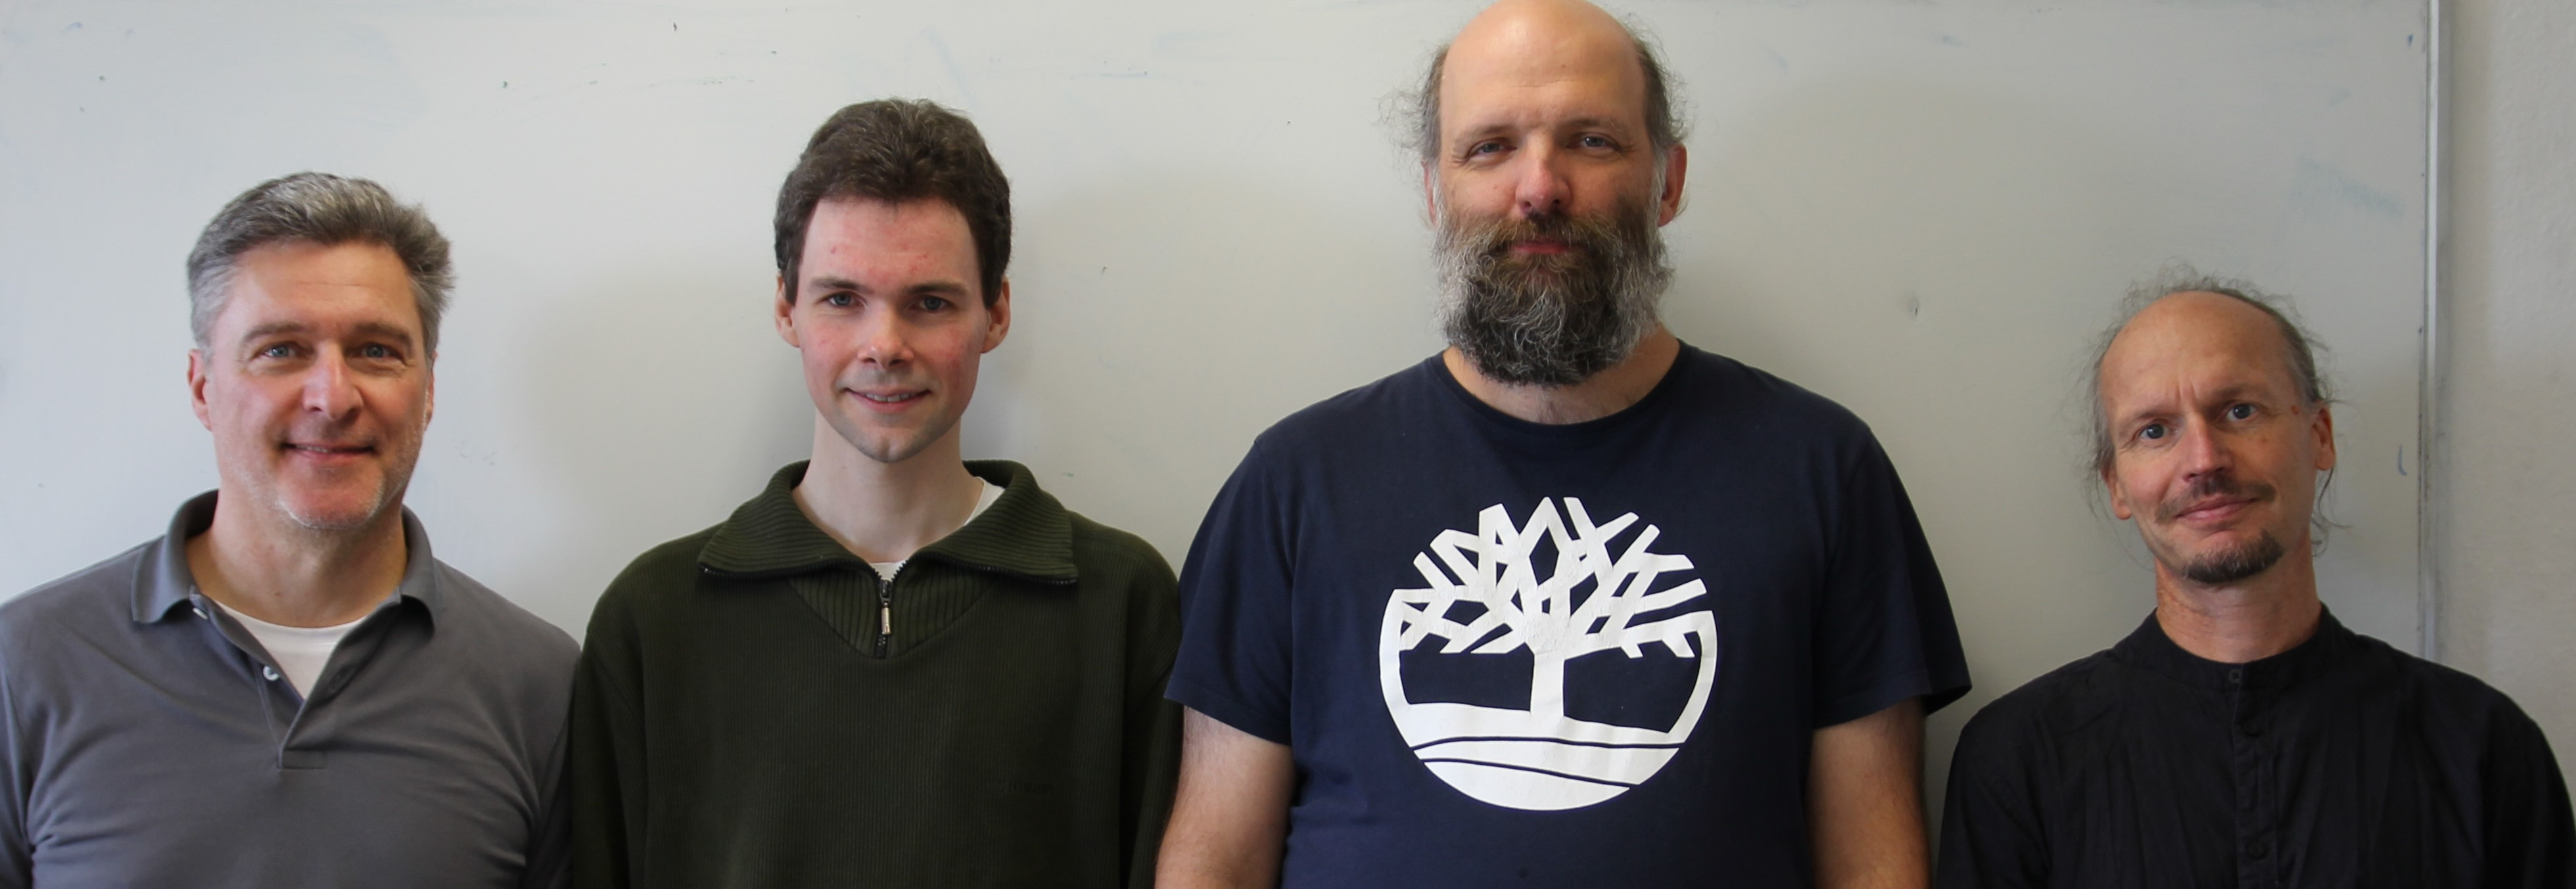
\includegraphics[width=0.6\columnwidth, height=0.25\textheight]{res/vorstellungsfotos/profs_ws23.jpg}\\
%\smallskip
%Gruppenfoto der Physik~1-3 Dozenten; in Ihrem Bezugssystem von links nach rechts: Carsten~Fallnich, Raphael~Wittkowski, Karol~Kovarik und Uwe~Thiele.
%\end{center}

\newpage

\begin{multicols}{2}

\begin{center} 
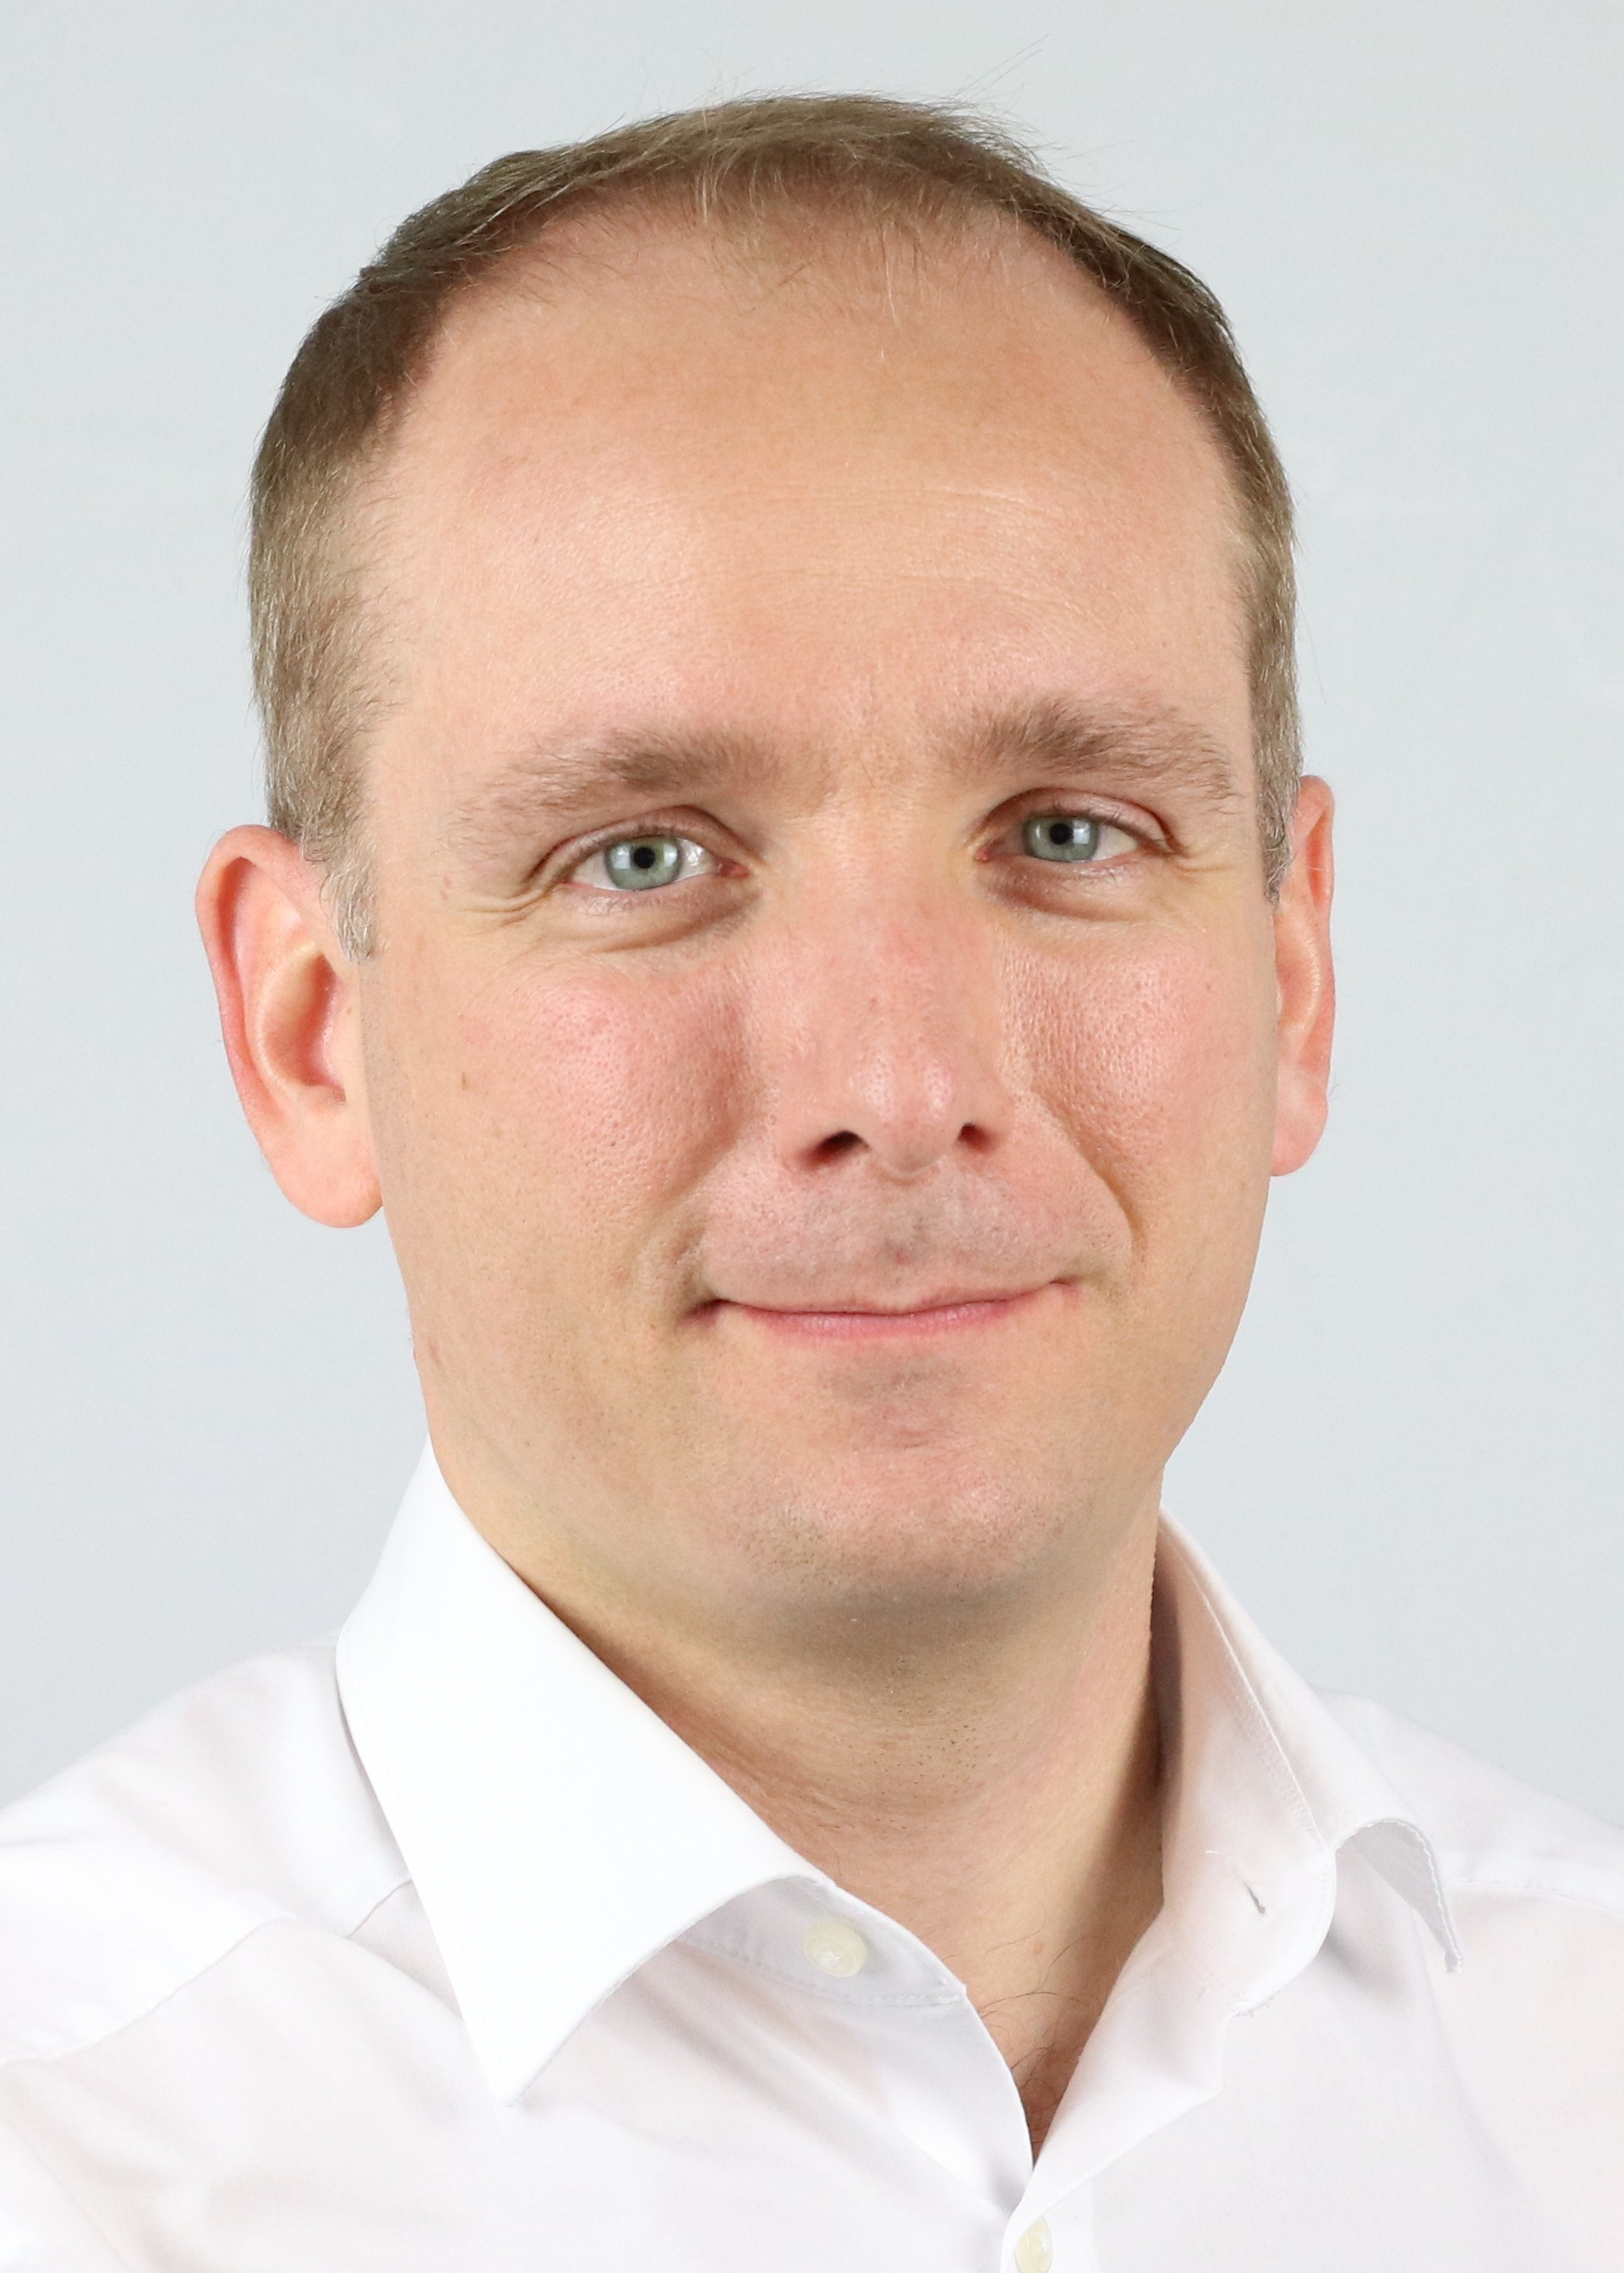
\includegraphics[width=0.8\columnwidth, height=0.25\textheight]{res/vorstellungsfotos/Foto_Salinga.jpg}
\smallskip
Prof.\ Dr.\ Martin Salinga\\ 
Institut für Theoretische Physik
\end{center} 

Gerne schließe ich mich meinem Kollegen, Michael Klasen, an: Herzlich willkommen an der Universität Münster! 

Neben dem befriedigenden Gefühl, etwas tiefgehend verstanden zu haben, motiviert mich bei meiner Arbeit als Physiker die Zuversicht, mit meinen Erkenntnissen zum technischen Fortschritt beitragen zu können. In meinem Forschungsgebiet interessieren wir uns für die physikalischen Eigenschaften von Materialien, woraus sie sich ergeben und wie sie nutzbar gemacht werden können. In meiner Arbeitsgruppe hier in Münster widmen wir Zustandsänderungen besondere Aufmerksamkeit, die sich zur Realisierung hocheffizienter Computerhardware anbieten. Dabei lassen wir uns von Funktionsprinzipien (natürlicher und künstlicher) neuronaler Netze inspirieren. 

Vor meiner Berufung auf die Professur im hiesigen Institut für Materialphysik im Jahr 2019 war ich lange Zeit an der Rheinisch-Westfälischen Technischen Hochschule in Aachen tätig, wo ich im Anschluss an meine Promotion im Jahr 2008 eine unbefristete Stelle annahm, mit vielfältigen Aufgaben in Forschung und Lehre. Darüber hinaus haben mich allerdings diverse Forschungsaufenthalte im Ausland geprägt; in Boston, in Zürich und im Silicon Valley in Kalifornien. Vor allem die Erfahrungen aus industriellen Forschungskontexten bei IBM empfinde ich als große Bereicherung. 
 
Genau 25 Jahre nachdem ich mein eigenes Physikstudium an der Rheinisch-Westfälischen Technischen Hochschule in Aachen begann, darf ich nun Sie in der Anfangsphase Ihres Physikstudiums begleiten. Ich freue mich auf vielfältige Begegnungen und wünsche Ihnen alles Gute für Ihren Studienstart!

%\begin{center}
%\includegraphics[width=0.8\columnwidth]{private/res/comics/manchmal_edited.jpg}\\
%{\footnotesize 
%S.~Harris – \url{sciencecartoonsplus.com}
%}
%\end{center}

\end{multicols}

\vfill

\newpage

\begin{multicols}{2}
\begin{center}
	% \includegraphics[width=\columnwidth, height=0.35\textheight]{res/vorstellungsfotos/wend_werner.jpg}\\
	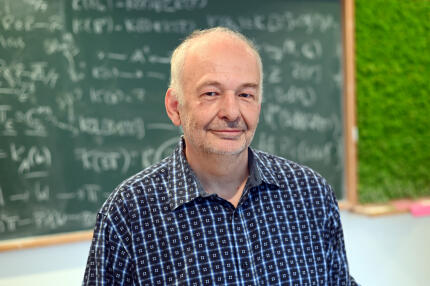
\includegraphics[width=\columnwidth, height=0.35\textheight]{res/vorstellungsfotos/Hille.jpg}\\
	\smallskip
 	Prof.\ Dr.\ Raimar Wulkenhaar\\
	Mathematisches Institut
\end{center}
Liebe Studentinnen und Studenten,

ich habe im WiSe 2024/25 die Aufgabe übernommen, die Vorlesung Mathematik für Physiker zu lesen, die eine für den Vorlesenden sehr anspruchsvolle Vorlesung ist. Hier wird versucht, die wichtigsten mathematischen Grundlagen zu vermitteln, aus dem inzwischen riesigen Reich der Mathematik und Physik muss dabei eine kleine Auswahl getroffen werden.

Ich selbst war bereits von Kindesbeinen an immer sehr an Mathematik und Physik, sowie Elektronik und Biologie interessiert. Nach meiner Schulzeit habe ich mich dann aber aus unterschiedlichen Gründen entschieden, Mathematik an der Humboldt-Universität zu studieren. Nach dem Studium habe ich in Bielefeld auf einem Gebiet der Darstellungstheorie promoviert und nach Stationen in Chemnitz, Hamburg mit Habilitation, Bielefeld, Bonn, Berlin und einigen kürzeren Auslandsaufenthalten hat es mich nach Münster verschlagen.

Hier arbeite ich jetzt auf der Verbindung zwischen Geometrie, Darstellungstheorie und Kombinatorik. Mein Interesse an physikalischen Fragen ist in letzter Zeit wieder stärker geworden, insbesondere versuche ich neuere Entwicklungen zu verfolgen und es gibt ein aktives Oberseminar zu geometrischen Fragen der Physik.

In der Vorlesung sehe ich es als meine Hauptaufgabe an, die Verbindung zwischen Linearer Algebra und Analysis soweit zu erklären, dass aufbauend darauf weitere mathematische Inhalte selbstständig erschlossen werden können. Dazu wird es neben der Vorlesung aktive Übungen geben. Mathematik ist einerseits natürlich Wissen, andererseits aber auch ein Teil Handwerk, und dann als Höhepunkt die Übertragung der Realität in Formeln und die Vorhersage der Realität mit Hilfe der Theorie. Ich werde versuchen diesen Teil immer wieder an physikalisch relevanten Beispielen erläutern, sodass die Stärke der Mathematik für die Physik auch sichtbar wird.

Wer gerne auch persönlich Kontakt sucht, findet mich beim Bouldern, auf dem Fahrrad, in netten Cafés oder beim Motorrad fahren. Letzteres dabei möglichst weit weg von Münster, zum Beispiel in Norwegen, in den Masuren, in Großbritannien oder Italien. Ich freue mich sehr, den Kurs Mathematik für Physiker lesen zu dürfen, es wird sicher anstrengend aber hoffentlich auch sehr erfolgreich.

Schlecht steht es um den Schüler, der seinen Meister nicht überflügelt.

In diesem Sinne freue ich mich auf meine neue Herausforderung, Ihre klugen Fragen und viele neue Erkenntnisse.

\[
\resizebox{0.45\hsize}{!}{$\displaystyle\sum_{n = 1}^\infty \frac{1}{n^2} = \frac{\pi^2}{6}$}
\]

\begin{center}
	%\fibelimgtext{
		%\includegraphics[width=0.85\textwidth]{res/xkcd/435_purity.png}
	%}{\url{https://xkcd.com/435}}
 	\includegraphics[width=0.85\columnwidth]{private/res/comics/calvin_mathe.pdf}
\end{center}

\end{multicols}
